\chapter{Opis projektnog zadatka}
		
		Cilj ovog projekta je razviti programsku podršku za web aplikaciju “Radno vrijeme” koja će omogućiti  djelatnicima poduzeća „Mi puno radimo“ praćenje realizacije pojedinih djelatnosti i radnih sati na razini svakog djelatnika, grupe i poduzeća, kao i praćenje zauzeća/raspoloživosti pojedinih djelatnika. Na taj će se način olakšati organizacija istovremenog obavljanja mnogih uslužnih djelatnosti.\\
		
		Korisnike sustava možemo podijeliti u 4 grupe: 
		\begin{itemize}
			\item vlasnika sustava
			\item voditelja grupa
			\item zaposlenike
			\item neregistrirane korisnike\\
		\end{itemize}
		
		Neregistrirani korisnici mogu samo vidjeti popis i opis djelatnosti koje poduzeće ima u svojem portfoliju. Direktoru je omogućeno registriranje korisnika u sustav kreiranjem novog računa. Za kreiranje novog računa potrebni su sljedeći podaci:
		\begin{itemize}
			\item korisničko ime
			\item lozinka
			\item ime
			\item prezime
			\item OIB
			\item adresa e-pošte\\
		\end{itemize} 
		
		Svim djelatnicima kasnije korisničko ime i lozinka služe za prijavu u sustav, a adresa e-pošte kako bi ih se moglo kontaktirati. \\
		
		Naknadno se djelatnicima, ako već nisu, mogu još i dodijeliti prava voditelja grupe. Ukoliko radnici idu na intervencije izvan lokacije sjedišta poduzeća, potrebno je za svakoga prikazati mjesto na karti za lokaciju na koju je bio upućen.\\ 
		
		Djelatnik poduzeća kroz aplikaciju  može vidjeti podatke samo o sebi. Njemu se prikazuju grupe u koje je raspodijeljen te zadatke koji su mu dodijeljeni. Jedan djelatnik može biti raspoređen i na nekoliko radnih zadataka unutar jedne djelatnosti, a i između više njih.\\
		
		Ukoliko je djelatniku dodijeljen zadatak na nekoj lokaciji različitoj od sjedišta poduzeća, on tu promjenu u lokaciji mora unijeti na karti prije odlaska, ako nije voditelj grupe već unio u sustav.\\
		
		Voditelji grupa mogu kroz aplikaciju dobiti podatke o sebi, ali i o članovima svoje grupe. Oni razrađuju plan rada svoje grupe te određuju zadatke i pridjeljuju ih zaposlenicima. Za svaki zadatak voditelj određuje očekivani broj potrebnih radnih sati te cijenu radnog sata na razini pojedine djelatnosti i/ili zadatka. \\
		
		Vlasnik može stvarati grupe, pri čemu zaposlenika postavlja kao voditelja te grupi dodjeljuje djelatnost i članove, a također ima mogućnost brisanja grupe.  
	
		On također može definirati nove uslužne djelatnosti kojima se poduzeće bavi te će te promjene biti vidljive u popisu djelatnosti.  
	
		Vlasniku sustava se kroz aplikaciju prikazuju zauzetost i realizacija (stvarna i materijalna) za sve djelatnike te odnos planiranih i realiziranih troškova/dobiti. Informacija o zauzetosti djelatnika pomaže mu pri stvaranju grupa kako ne bi preopteretio zaposlenike prevelikom količinom zadataka te na taj način osigurao veću količinu i kvalitetu odrađenog posla. 
	
		Ukoliko postoje aktivnosti izvan sjedišta poduzeća, direktor u svakom trenutku mora moći vidjeti na karti gdje se nalazi (ili se nalazio) koji djelatnik. Podaci o adresi intervencije moraju biti prethodno uneseni u sustav. \\
		
		Na kraju svakog radnog dana svaki pojedini djelatnik (uključujući i voditelje grupa) upisuju broj odrađenih radnih sati taj dan.\\
		
		Sustav mora omogućiti istovremeni rad svih korisnika sustava i mora omogućiti unos hrvatskih dijakritičkih znakova.\\
		
		Sustav također mora biti prilagođen i u potpunosti poštivati sva prava radnika, uključujući radno vrijeme (početak i kraj), duljinu radnog vremena, slobodne dana i ostala prava koja radnik ima temeljem općih i posebnih uvjeta definiranih zakonom.\\
		
		Gledajući dostupne programe koji bi omogućili praćenje produktivnosti zaposlenika  možemo vidjeti razne kategorije. Od najpopularinijih, najskupljih, najjednostavnijih pa sve do najjeftinijih. Ujedno je problem što je toliko veliki izbor između svih programa. To otežava voditeljima poduzeća posao odmjeravanja jakosti i slabosti svakog programa. Pošto su svi ti programi namjenjeni široj publici, svaki od tih programa će doći sa svojim opcijama koje nisu nužne niti potrebne poduzeću "Mi puno radimo".
		Ukoliko odaberu neki program, tu dolazi još jedan problem. Učenje korištenja tog programa (engl. \textit{learning curve)}. Potrebno je vrijeme i trud prije nego što počnu koristiti taj program optimizirano.\\
		
		Tu dolazimo mi. Mi dajemo priliku poduzeću "Mi puno radimo" sa krojenim programom prema njihovim potrebama. Ne trebaju plaćati za opcije koje neće koristiti, ne trebaju odustati od svojih zahtjeva kako bi koristili jeftinija i/ili lošija rješenja. Dajemo im priliku da napravimo program koji će oni sami intuitivno znati koristiti jer će sudjelovati u svakom koraku korisničkog sučelja i njegovih funkcionalnosti.\\ 
		
		Projekt je uvijek moguće nadograditi. Ovaj projekt je savršen za male, srednje i velike tvrtke. Možemo uz dogovor s klijentima povezati program s njihovim drugim servisima za koje drugi programi nemaju mogućnost, a niti im je u planu jer većina ne bi koristila. Trenutni cilj projekta nije specifičan da ga može samo jedno poduzeće koristiti. Na primjer, trenutna ideja je da zaposlenici sami unesu broj radnih sata za pojedini dan, moguće je nadograditi da se to automatski računa uz pametne kartice, opcionalno koje bismo mi enkriptirali. Također, ukoliko neke tvrtke imaju već brojače sati za zaposlenike, ali im treba većina naših opcija, uz dogovor možemo proširiti naš program da dobije podatke iz njihovog brojača te samo proširimo program za te servise koje oni traže.\\
		
		Prednost našeg rješenja je što ne zahtjeva instalaciju na svaki uređaj koji treba pristupiti servisu. Svatko može sa svojeg pametnog mobitela ili računala doći do svojih zadataka, preinaka i novih informacija. Samo trebaju znati svoje korisničko ime i lozinku. Iako ova prednost može doći kao i mana, tu opet dolazimo do naše prethodne snage. Mi možemo, ukoliko je potrebno, ojačati sigurnost programa. Na način da program dozvoli pristup samo ovlaštenim računalima/mobitelima. Na primjer, zabrana pristupa osim dozvoljenim MAC adresama, dozvola pristupa računalima i mobitelima sa instaliranim certifikatom koji mi napišemo i sl. Naša tvrtka kroji proizvod svojim klijentima.
		%\begin{packed_item}
		%	\item \textit{potencijalna korist ovog projekta}
		%	\item \textit{postojeća slična rješenja (istražiti i ukratko opisati razlike u odnosu na zadani zadatak). Dodajte slike koja predočavaju slična rješenja.}
		%	\item \textit{skup korisnika koji bi mogao biti zainteresiran za ostvareno rješenje.}
		%	\item \textit{mogućnost prilagodbe rješenja }
		%	\item \textit{opseg projektnog zadatka}
		%	\item \textit{moguće nadogradnje projektnog zadatka}
		%\end{packed_item}
		
		%\textit{Za pomoć pogledati reference navedene u poglavlju „Popis literature“, a po potrebi konzultirati sadržaj na internetu koji nudi dobre smjernice u tom pogledu.}
		\eject
		
		%\section{Primjeri u \LaTeX u}
		
		%\textit{Ovo potpoglavlje izbrisati.}\\

		%U nastavku se nalaze različiti primjeri kako koristiti osnovne funkcionalnosti \LaTeX a koje su potrebne za izradu dokumentacije. Za dodatnu pomoć obratiti se asistentu na projektu ili potražiti upute na sljedećim web sjedištima:
		%\begin{itemize}
			%\item Upute za izradu diplomskog rada u \LaTeX u - \url{https://www.fer.unizg.hr/_download/repository/LaTeX-upute.pdf}
			%\item \LaTeX\ projekt - \url{https://www.latex-project.org/help/}
			%\item StackExchange za Tex - %\url{https://tex.stackexchange.com/}\\
		
		%\end{itemize} 	


		
		%\noindent \underbar{podcrtani tekst}, \textbf{podebljani tekst}, 	\textit{nagnuti tekst}\\
		%\noindent \normalsize primjer \large primjer \Large primjer \LARGE {primjer} \huge {primjer} \Huge primjer \normalsize
				
		%\begin{packed_item}
			
			%\item  primjer
			%\item  primjer
			%\item  primjer
			%\item[] \begin{packed_enum}
			%	\item primjer
			%	\item[] \begin{packed_enum}
			%		\item[1.a] primjer
			%		\item[b] primjer
			%	\end{packed_enum}
			%	\item primjer
			%\end{packed_enum}
			
		%\end{packed_item}
		
		%\noindent primjer url-a: \url{https://www.fer.unizg.hr/predmet/proinz/projekt}
		
		%\noindent posebni znakovi: \# \$ \% \& \{ \} \_ 
		%$|$ $<$ $>$ 
		%\^{} 
		%\~{} 
		%$\backslash$ 
		
		%\begin{longtabu} to \textwidth {|X[8, l]|X[8, l]|X[16, l]|} %definicija širine tablice, širine stupaca i poravnanje
			
		%	%definicija naslova tablice
		%	\hline \multicolumn{3}{|c|}{\textbf{naslov unutar tablice}}	 \\[3pt] \hline
		%	\endfirsthead
			
			%definicija naslova tablice prilikom prijeloma
		%	\hline \multicolumn{3}{|c|}{\textbf{naslov unutar tablice}}	 \\[3pt] \hline
		%	\endhead
			
		%	\hline 
		%	\endlastfoot
			
		%	\rowcolor{LightGreen}IDKorisnik & INT	&  	Lorem ipsum dolor sit amet, consectetur adipiscing elit, sed do eiusmod  	\\ \hline
		%	korisnickoIme	& VARCHAR &   	\\ \hline 
		%	email & VARCHAR &   \\ \hline 
		%	ime & VARCHAR	&  		\\ \hline 
		%	\cellcolor{LightBlue} primjer	& VARCHAR &   	\\ \hline 
			
		%\end{longtabu}
		

		%\begin{table}[H]
			
		%	\begin{longtabu} to \textwidth {|X[8, l]|X[8, l]|X[16, l]|} 
				
		%		\hline 
		%		\endfirsthead
				
		%		\hline 
		%		\endhead
				
		%		\hline 
		%		\endlastfoot
				
		%		\rowcolor{LightGreen}IDKorisnik & INT	&  	Lorem ipsum dolor sit amet, consectetur adipiscing elit, sed do eiusmod  	\\ \hline
		%		korisnickoIme	& VARCHAR &   	\\ \hline 
		%		email & VARCHAR &   \\ \hline 
		%		ime & VARCHAR	&  		\\ \hline 
		%		\cellcolor{LightBlue} primjer	& VARCHAR &   	\\ \hline 
				
				
		%	\end{longtabu}
	
		%	\caption{\label{tab:referencatablica} Naslov ispod tablice.}
		%\end{table}
		
		
		%unos slike
		%\begin{figure}[H]
		%	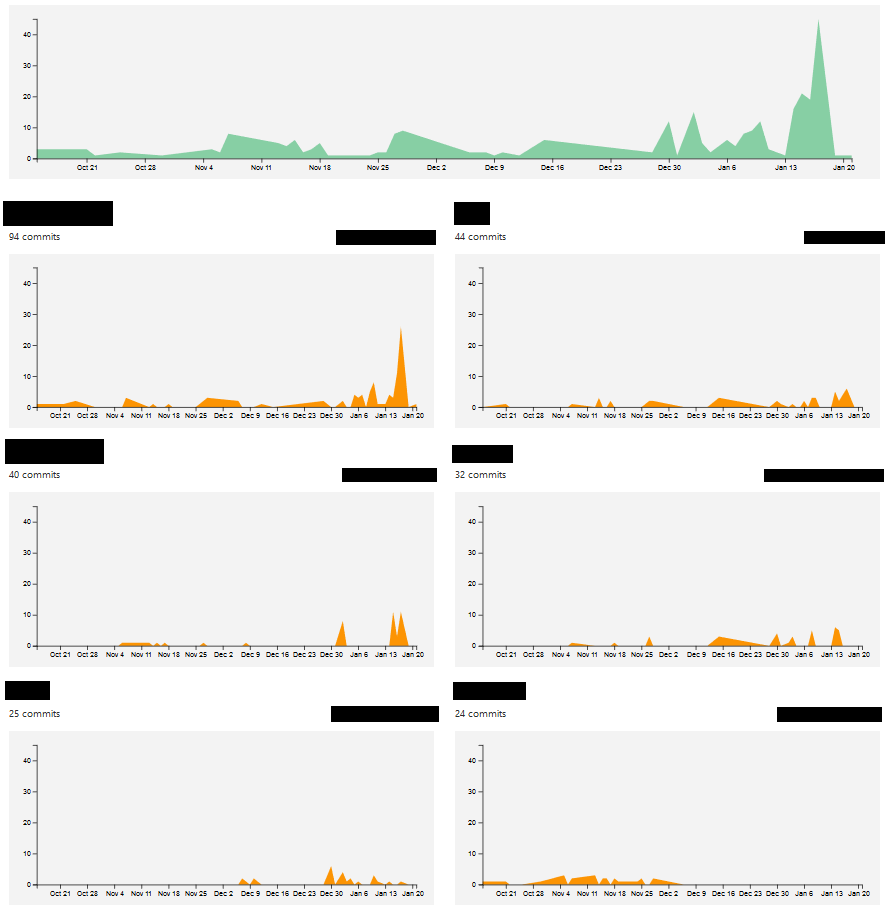
\includegraphics[scale=0.4]{slike/aktivnost.PNG} %veličina slike u odnosu na originalnu datoteku i pozicija slike
		%	\centering
		%	\caption{Primjer slike s potpisom}
		%	\label{fig:promjene}
		%\end{figure}
		
		%\begin{figure}[H]
		%	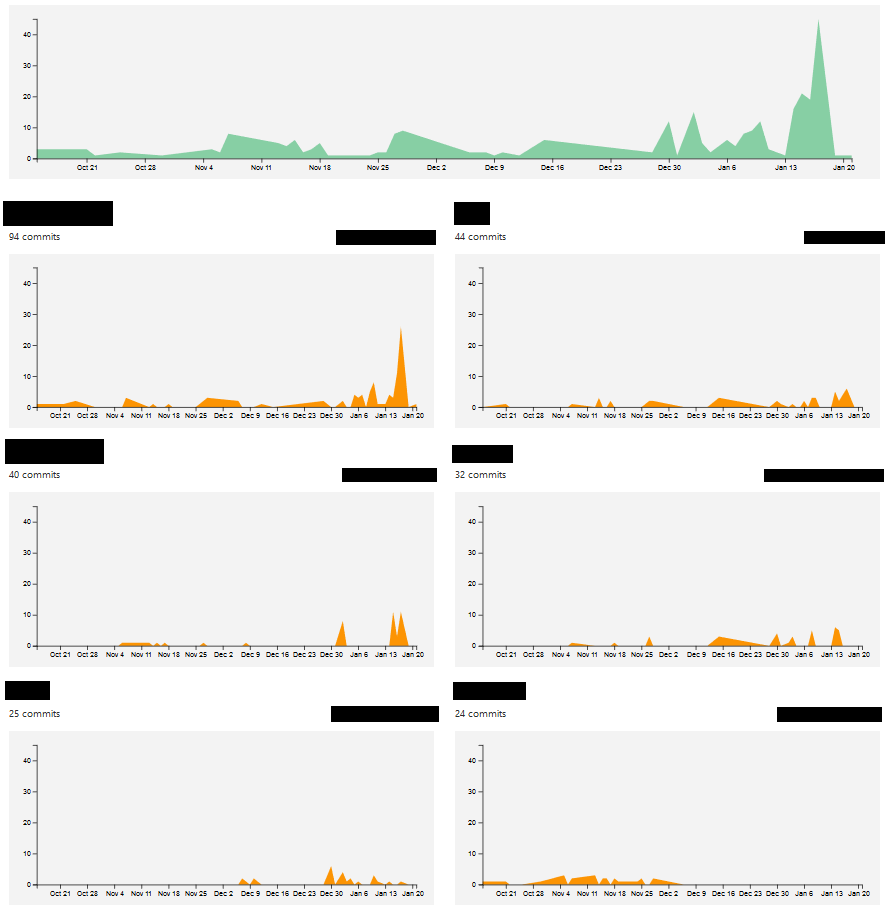
\includegraphics[width=.9\linewidth]{slike/aktivnost.PNG} %veličina u odnosu na širinu linije
		%	\caption{Primjer slike s potpisom 2}
		%	\label{fig:promjene2} %label mora biti drugaciji za svaku sliku
		%\end{figure}
		
		%Referenciranje slike \ref{fig:promjene2} u tekstu.
		
		\eject
		
	